\documentclass[aspectratio=169,xcolor={dvipsnames,table}]{beamer}
\usepackage[no-math,deluxe,haranoaji]{luatexja-preset}
\renewcommand{\kanjifamilydefault}{\gtdefault}
\renewcommand{\emph}[1]{{\upshape\bfseries #1}}
\usetheme{metropolis}
\metroset{block=fill}
\setbeamertemplate{navigation symbols}{}
\setbeamertemplate{blocks}[rounded][shadow=false]
\usecolortheme[rgb={0.7,0.2,0.2}]{structure}
%%%%%%%%%%%%%%%%%%%%%%%%%%
%% Change alert block colors
%%% 1- Block title (background and text)
\setbeamercolor{block title alerted}{fg=mDarkTeal, bg=mLightBrown!45!yellow!45}
\setbeamercolor{block title example}{fg=magenta!10!black, bg=mLightGreen!70}
%%% 2- Block body (background)
\setbeamercolor{block body alerted}{bg=mLightBrown!25}
\setbeamercolor{block body example}{bg=mLightGreen!15}
%%%%%%%%%%%%%%%%%%%%%%%%%%%
%%%%%%%%%%%%%%%%%%%%%%%%%%%
%% さまざまなアイコン
%%%%%%%%%%%%%%%%%%%%%%%%%%%
%\usepackage{fontawesome}
\usepackage{fontawesome5}
\usepackage{figchild}
\usepackage{twemojis}
\usepackage{utfsym}
\usepackage{bclogo}
\usepackage{marvosym}
\usepackage{fontmfizz}
\usepackage{pifont}
\usepackage{phaistos}
\usepackage{worldflags}
\usepackage{jigsaw}
\usepackage{tikzlings}
\usepackage{tikzducks}
\usepackage{scsnowman}
\usepackage{epsdice}
\usepackage{halloweenmath}
\usepackage{svrsymbols}
\usepackage{countriesofeurope}
\usepackage{tipa}
\usepackage{manfnt}
%%%%%%%%%%%%%%%%%%%%%%%%%%%
\usepackage{tikz}
\usetikzlibrary{calc,patterns,decorations.pathmorphing,backgrounds}
\usepackage{tcolorbox}
\usepackage{tikzpeople}
\usepackage{circledsteps}
\usepackage{xcolor}
\usepackage{amsmath}
\usepackage{booktabs}
\usepackage{chronology}
\usepackage{signchart}
%%%%%%%%%%%%%%%%%%%%%%%%%%%
%% 場合分け
%%%%%%%%%%%%%%%%%%%%%%%%%%%
\usepackage{cases}
%%%%%%%%%%%%%%%%%%%%%%%%%%
\usepackage{pdfpages}
%%%%%%%%%%%%%%%%%%%%%%%%%%%
%% 音声リンク表示
\newcommand{\myaudio}[1]{\href{#1}{\faVolumeUp}}
%%%%%%%%%%%%%%%%%%%%%%%%%%
%% \myAnch{<名前>}{<色>}{<テキスト>}
%% 指定のテキストを指定の色の四角枠で囲み, 指定の名前をもつTikZの
%% ノードとして出力する. 図には remember picture 属性を付けている
%% ので外部から参照可能である.
\newcommand*{\myAnch}[3]{%
  \tikz[remember picture,baseline=(#1.base)]
    \node[draw,rectangle,line width=1pt,#2] (#1) {\normalcolor #3};
}
%%%%%%%%%%%%%%%%%%%%%%%%%%
%% \myEmph コマンドの定義
%%%%%%%%%%%%%%%%%%%%%%%%%%
%\newcommand{\myEmph}[3]{%
%    \textbf<#1>{\color<#1>{#2}{#3}}%
%}
\usepackage{xparse} % xparseパッケージの読み込み
\NewDocumentCommand{\myEmph}{O{} m m}{%
    \def\argOne{#1}%
    \ifx\argOne\empty
        \textbf{\color{#2}{#3}}% オプション引数が省略された場合
    \else
        \textbf<#1>{\color<#1>{#2}{#3}}% オプション引数が指定された場合
    \fi
}
%%%%%%%%%%%%%%%%%%%%%%%%%%%
%%%%%%%%%%%%%%%%%%%%%%%%%%%
%% 文末の上昇イントネーション記号 \myRisingPitch
%% 通常のイントネーション \myDownwardPitch
%% https://note.com/dan_oyama/n/n8be58e8797b2
%%%%%%%%%%%%%%%%%%%%%%%%%%%
\newcommand{\myRisingPitch}{
\begin{tikzpicture}[scale=0.3,baseline=0.3]
\draw[->,>=stealth] (0,0) to[bend right=45] (1,1);
\end{tikzpicture}
}
\newcommand{\myDownwardPitch}{
\begin{tikzpicture}[scale=0.3,baseline=0.3]
\draw[->,>=stealth] (0,1) to[bend left=45] (1,0);
\end{tikzpicture}
}
%%%%%%%%%%%%%%%%%%%%%%%%%%%%
%\AtBeginSection[%
%]{%
%  \begin{frame}[plain]\frametitle{授業の流れ}
%     \tableofcontents[currentsection]
%   \end{frame}%
%}

\usepackage{pxrubrica}
\usetikzlibrary{tikzmark}
%%%%%%%%%%%%%%%%%%%%%%%%%%
\UseTblrLibrary{counter} %% added this line
%%%%%%%%%%%%%%%%%%%%%%%%%%%
\title{English is fun.}
\subtitle{I will give you some flowers.}
\author{}
\institute[]{}
\date[]

%%%%%%%%%%%%%%%%%%%%%%%%%%%%
%% TEXT
%%%%%%%%%%%%%%%%%%%%%%%%%%%%
\begin{document}


\begin{frame}[plain]
  \titlepage
\end{frame}


\section*{授業の流れ}
\begin{frame}[plain]
  \frametitle{授業の流れ}
  \tableofcontents
\end{frame}
%%%%%%%%%%%%%%%%%%%%%%%%%%%%%
 \section{give \textipa{/g\'Iv/}}
\begin{frame}[plain]{give $+$ 人 $+$ もの}
 \begin{enumerate}
  \item<1-> Birds sing. (SV)
  \item<2-> They speak English. (SVO)
  \item<3-> Cows \textbf{give} us milk. (SVOO)
 \end{enumerate}

\begin{block}<4->{Topics for Today}\small
 \textbf{give}(与える)は目的語を2つとります
\begin{itemize}\setbeamertemplate{items}[square]\small
 \item \textbf{give} $+$ \tikzmark{x}\Circled[fill color = white]{\,人\,} $+$ \tikzmark{y}\Circled[fill color = white]{\,もの\,}\hspace{20pt}「\ldots{}に~をあげる」\\
\hfill\tikzmark{X}{\scriptsize 間接目的語}\\
\hfill\tikzmark{Y}{\scriptsize 直接目的語}
 \item<5-> \begin{tblr}{
         colspec=llll,
         row{odd} = {bg=azure8},
         row{1} = {bg=azure3, fg=white},
         row{even} = {bg=white},
         baseline=c,
         hline{1,Z} = {0.08em},
         hline{2} = {0.05em}
 }
原形&過去形&過去分詞&ing\\
{give \textipa{/g\'Iv/}}&{gave \textipa{/g\'eIv/}}&{given \textipa{/g\'Ivn/}}&{giving \textipa{/g\'IvIN/}}
       \end{tblr}
\end{itemize}
\end{block}

\begin{tikzpicture}[remember picture,overlay]
 \visible<4->{\draw[<-] ([xshift=9pt,yshift=-4pt]pic cs:x) |- ([xshift=-2pt, yshift=2pt] pic cs:X);}
 \visible<4->{\draw[<-] ([xshift=14pt,yshift=-4pt]pic cs:y) |- ([xshift=-2pt, yshift=2pt] pic cs:Y);}
\end{tikzpicture}
\hfill{\scriptsize \myaudio{./audio/052_svoo_01.mp3}}
\end{frame}
%%%%%%%%%%%%%%%%%%%%%%%%%%%%%%%%%%
\begin{frame}[plain]{Exercises}

{\small 日本語の意味になるようカッコ内の語句を並べかえましょう。
文頭の語は大文字で始めてください}%
\mbox{}\hfill{\scriptsize \myaudio{./audio/052_svoo_02.mp3}}

 \begin{enumerate}
  \item {\small わたしは彼におもちゃをあげよう。} ( will / him / toy / I / give / a )\\
\visible<2->{I will give him a toy.}
  \item {\small 彼女は母親に花をあげた。} ( her / some / gave / flowers / mother / she )\\
\visible<3->{She gave her mother some flowers.}
  \item {\small おじがわたしにその本をくれました。} ( the / my / me / gave / book / uncle )\\
\visible<4->{My uncle gave me the book}.
  \item {\small その川は我々に水を供給してくれる。} ( gives / water / the / us / river )\\
\visible<5->{The river gives us water.}
 \end{enumerate}
\end{frame}
%%%%%%%%%%%%%%%%%%%%%%%
\section{giveのなかまたち1}
\begin{frame}[plain]{giveのなかまたち1}\large
 \begin{enumerate}
  \item<1-> I will \textbf{give} you a present.%
       \hfill{\scriptsize present \textipa{/pr\'eznt/} 贈り物}
  \item<2-> I will \textbf{send} you a present.
  \item<3-> I will \textbf{show} you the picture.%
       \hfill{\scriptsize picture \textipa{/p\'IktS\textrhookschwa /} 絵、写真}
  \item<4-> I will \textbf{write} you a letter.
  \item<5-> i will \textbf{tell} you a secret.%
       \hfill{\scriptsize secret \textipa{/s\'\i:kl@t/} 秘密}
  \item<6-> I will \textbf{teach} you history.%
       \hfill{\scriptsize history \textipa{/h\'Istri/} 歴史}

 \end{enumerate}

\begin{block}<7->{S $+$ V $+$ O $+$ O\hfill{\scriptsize \myaudio{./audio/052_svoo_03.mp3}}}\small
$\left\{ \begin{tabular}{l}
%	  give\\
	  send\\
	  show\\
	  write\\
	  tell\\
	  teach\\
	 \end{tabular}\right\} + \tikzmark{a}\text{\Circled[fill color=white]{\,人\,}} + \tikzmark{b}\text{\Circled[fill color=white]{\,もの・こと\,}}$

\hfill\tikzmark{A}{\scriptsize 間接目的語}\\
\hfill\tikzmark{B}{\scriptsize 直接目的語}
\end{block}

\begin{tikzpicture}[remember picture,overlay]
 \visible<7->{\draw[<-] ([xshift=9pt,yshift=-4pt]pic cs:a) |- ([xshift=-2pt, yshift=2pt] pic cs:A);}
 \visible<7->{\draw[<-] ([xshift=24pt,yshift=-4pt]pic cs:b) |- ([xshift=-2pt, yshift=2pt] pic cs:B);}
\end{tikzpicture}
\end{frame}
%%%%%%%%%%%%%%%%%%%%%%%%%%%%%%%
\begin{frame}[plain]{一覧表}
  \begin{tblr}{
         colspec=llll,
         row{odd} = {bg=azure8},
         row{1} = {bg=azure3, fg=white},
         row{even} = {bg=white},
         row{2} = {bg=white},
         baseline=c,
         hline{1,Z} = {0.08em},
         hline{2} = {0.05em},
         cells={cmd=\onslide<\arabic{colnum}->} %列ごとに順次表示%%%tabularrayとpauseが衝突することを回避する方法→https://github.com/lvjr/tabularray/issues/226
}
原形&過去形&過去分詞&ing\\
give \textipa{/g\'Iv/}&gave \textipa{/g\'eIv/}&given \textipa{/g\'Ivn/}&giving \textipa{/g\'IvIN/}\\
send \textipa{/s\'end/}&sent \textipa{/s\'ent/}&sent \textipa{/s\'ent/}&sending \textipa{/s\'endiN/}\\
show \textipa{/S\'oU/}&showed \textipa{/S\'oUd/}&shown \textipa{/S\'oUn/}&showing \textipa{/S\'oUiN/}\\
write \textipa{/r\'aIt/}&wrote \textipa{/r\'oUt/}&written \textipa{/r\'Itn/}&writing \textipa{/r\'aItiN/}\\
tell \textipa{/t\'el/}&told \textipa{/t\'oUld/}&told \textipa{/t\'oUld/}&telling \textipa{/t\'eliN/}\\
teach \textipa{/t\'\i:tS/}&taught \textipa{/t\'O:t/}&taught \textipa{/t\'O:t/}& teaching \textipa{/t\'\i:tSiN/}
       \end{tblr}

\hfill{\scriptsize \myaudio{./audio/052_svoo_04.mp3}}
\end{frame}
%%%%%%%%%%%%%%%%%%%%%%%%%%%%%%%
\begin{frame}[plain]{Exercises}{}

{\small 日本語の意味になるようカッコ内の語句を並べかえましょう}
 \hfill{\scriptsize \myaudio{./audio/052_svoo_05.mp3}}


\begin{enumerate}
 \item {\small 私にその写真を見せてください。}  Please ( picture / me  / the / show ). \\
       \visible<2->{Please show me the picture.}
 \item {\small 彼女は先月彼に手紙を送りました。}
She ( a / him / month / sent / letter / last )\\
\visible<3->{She sent him a letter last month.}
 \item {\small 私は彼に手紙を毎週書きます。} I ( week / him / a / write / letter / every )\\
\visible<4->{I write hime a letter every week}.
 \item {\small 父は毎晩わたしにおもしろい話をしてくれます。}\\
My ( me / story / tells / night / interesting / an / every / father )\\
\visible<5->{My father tells me an interesting story every night.}
 \item {\small きのうJanisは彼らに新しい歌を教えた}。\\
Janis ( yesterday / a / taught / song / them / new )\\
\visible<6->{Janis taught them a new song yesterday.}
\end{enumerate}

\end{frame}
%%%%%%%%%%%%%%%%%%%%%%%%%%%%%%%%
\section{giveのなかまたち2}
\begin{frame}[plain]{giveのなかまたち2}\large
\begin{enumerate}
 \item<1-> I will \textbf{buy} you chocolate.%
\hfill{\scriptsize chocolate \textipa{/tS\'Akl@t/} チョコレート}
 \item<2-> I will \textbf{make} her a chair.
 \item<3-> I will \textbf{cook} them lunch.
\end{enumerate}


\begin{block}<4->{これもS $+$ V $+$ O $+$ O}\small

$\left\{ \begin{tabular}{l}
%	  give\\
	  buy\\
	  make\\
	  cook\\
	 \end{tabular}\right\} + \tikzmark{c}\text{\Circled[fill color=white]{\,人\,}} + \tikzmark{d}\text{\Circled[fill color=white]{\,もの\,}}$

\hfill\tikzmark{C}{\scriptsize 間接目的語}\\
\hfill\tikzmark{D}{\scriptsize 直接目的語}
\end{block}

\begin{tikzpicture}[remember picture,overlay]
 \visible<4->{\draw[<-] ([xshift=9pt,yshift=-4pt]pic cs:c) |- ([xshift=-2pt, yshift=2pt] pic cs:C);}
 \visible<4->{\draw[<-] ([xshift=12pt,yshift=-4pt]pic cs:d) |- ([xshift=-2pt, yshift=2pt] pic cs:D);}
\end{tikzpicture}

\hfill{\scriptsize \myaudio{./audio/052_svoo_06.mp3}}
\end{frame}
%%%%%%%%%%%%%%%%%%%%%%%%%%%%%
\begin{frame}[plain]{一覧表}
  \begin{tblr}{
         colspec=llll,
         row{odd} = {bg=azure8},
         row{1} = {bg=azure3, fg=white},
         row{even} = {bg=white},
         row{2} = {bg=white},
         baseline=c,
         hline{1,Z} = {0.08em},
         hline{2} = {0.05em},
         cells={cmd=\onslide<\arabic{colnum}->} %列ごとに順次表示%%%tabularrayとpauseが衝突することを回避する方法→https://github.com/lvjr/tabularray/issues/226
}
原形&過去形&過去分詞&ing\\
buy \textipa{/b\'aI/}&bought \textipa{/b\'O:t/}&bought \textipa{/b\'O:t/}&buying \textipa{/b\'aIIN/}\\
make \textipa{/m\'eIk/}&made \textipa{/m\'eId/}&made \textipa{/m\'eId/}&making \textipa{/m\'eIkiN/}\\
cook \textipa{/k\'Uk/}&cooked \textipa{/k\'Ukt/}&cooked \textipa{/k\'Ukt/}&cooking \textipa{/k\'UkiN/}\\
       \end{tblr}

\hfill{\scriptsize \myaudio{./audio/052_svoo_07.mp3}}
\end{frame}
%%%%%%%%%%%%%%%%%%%%%%%%%%%
%%%%%%%%%%%%%%%%%%%%%%%%%%%%%%%
\begin{frame}[plain]{Exercises}

{\small 日本語の意味になるようカッコ内の語句を並べかえましょう。先頭の語は大文字で始めてください}
 \hfill{\scriptsize \myaudio{./audio/052_svoo_08.mp3}}
\begin{enumerate}
 \item {\small 彼は昨日、私たちにおいしい食事を作ってくれました。}\\
       ( us / he / a delicious meal / cooked ) yesterday.\\
       \visible<2->{He cooked us a delicious meal yesterday.}
 \item {\small 彼女はわたしに素敵な時計を買ってくれました。}\\
       ( watch / bought / nice / me / a / she ).\\
       \visible<3->{She bought me a nice watch.}
 \item {\small わたしは明日彼らにケーキを作ります。}\\
( will / tomorrow / them / I / a cake / make ).\\
       \visible<4->{I will make them a cake tomorrow.}
\end{enumerate}
\end{frame}
%%%%%%%%%%%%%%%%%%%%%%%%%%%%%%%%

\begin{frame}[plain]{Exercises}
\small
\begin{tcolorbox}[colframe=ForestGreen,
  colback=ForestGreen!10!white,
  colbacktitle=ForestGreen!40!white,
  coltitle=black, %fonttitle=\bfseries,
  before upper={\setlength{\parindent}{1.5em}},
  title=英文を読んで、問に答えましょう\hfill{\scriptsize \myaudio{./audio/052_svoo_09.mp3}}
]
Betty loved\tikzmark{clue1} science. She wanted to help the Earth.
For her school project, she made a simple water filter.
She made clean water from a dirty bottle and gave it to her classmates.
Everyone was surprised\footnote{\scriptsize surprised おどろいた}. 
Her teacher said, ``You showed us a great idea!''
Betty smiled.

The next day, her tea\tikzmark{clue2}cher gave Betty a science award\footnote{\scriptsize award 賞}.
She was surprised and happy.
``I want to teach people how to make\footnote{\scriptsize how to make ~のつくり方} clean\tikzmark{clue3} water easily.''
Science gave her not only knowledge, but a big\tikzmark{clue4} dream, too.
\end{tcolorbox}

\vspace{-5pt}

\begin{enumerate}\scriptsize\setlength{\itemsep}{-2pt}
 \item<2-> Bettyは理科が好きですか、それともきらいですか\tikzmark{q1}\hfill\visible<4->{とても好き}
 \item<2-> だれがBettyに賞をあげましたか\tikzmark{q2}\hfill\visible<6->{彼女の先生}
 \item<2-> Bettyは人々に何を教えてあげたいとおもっていますか\tikzmark{q3}\hfill\visible<8->{かんたんにきれいな水をつくる方法}
 \item<2-> 理科はBettyに知識以外に何をあたえてくれましたか\tikzmark{q4}\hfill\visible<10->{おおきな夢}

\end{enumerate}


\begin{tikzpicture}[remember picture,overlay]
 \visible<3->{\draw[<-,opacity=0.4,line width=2pt] ([yshift=-2pt]pic cs:clue1) to[bend left] ([xshift=2pt, yshift=2pt] pic cs:q1);}
 \visible<5->{\draw[<-,opacity=0.4,line width=2pt] ([yshift=-2pt]pic cs:clue2) to[bend right] ([xshift=2pt, yshift=2pt] pic cs:q2);}
 \visible<7->{\draw[<-,opacity=0.4,line width=2pt] ([yshift=-2pt]pic cs:clue3) to ([xshift=2pt, yshift=2pt] pic cs:q3);}
 \visible<9->{\draw[<-,opacity=0.4,line width=2pt] ([yshift=-2pt]pic cs:clue4) to ([xshift=2pt, yshift=2pt] pic cs:q4);}
\end{tikzpicture}
\end{frame}
%%%%%%%%%%%%%%%%%%%%%%%%%%%%%%%
\section{まとめ}
\begin{frame}[plain]{まとめ}

\begin{block}{S $+$ V $+$ O $+$ O}\small
 \textbf{give}(与える)は目的語を2つとります
\begin{itemize}\setbeamertemplate{items}[square]\small
 \item \textbf{give} $+$ \tikzmark{aa}\Circled[fill color = white]{\,人\,} $+$ \tikzmark{bb}\Circled[fill color = white]{\,もの\,}\hspace{20pt}「\ldots{}に~をあげる」\\
\hfill\tikzmark{AA}{\scriptsize 間接目的語     }\\
\hfill\tikzmark{BB}{\scriptsize 直接目的語}
 \item giveのなかまたち\\
$\left\{ \begin{tabular}{l}
%	  give\\
	  send\\
	  show\\
	  write\\
	  tell\\
	  teach\\
	  buy\\
	  make\\
	  cook\\
	 \end{tabular}\right\} + \tikzmark{aaa}\text{\Circled[fill color=white]{\,人\,}} + \tikzmark{bbb}\text{\Circled[fill color=white]{\,もの・こと\,}}$
\end{itemize}
\end{block}

\begin{tikzpicture}[remember picture,overlay]
 \visible{\draw[<-] ([xshift=9pt,yshift=-4pt]pic cs:aa) |- ([xshift=-2pt, yshift=2pt] pic cs:AA);}
 \visible{\draw[<-] ([xshift=14pt,yshift=-4pt]pic cs:bb) |- ([xshift=-2pt, yshift=2pt] pic cs:BB);}
 \visible{\draw[<-] ([xshift=9pt,yshift=-4pt]pic cs:aaa) -- ([xshift=9pt,yshift=-14pt]pic cs:aaa)-- ([xshift=9pt,yshift=-14pt]pic cs:aaa) -| ([xshift=12pt, yshift=-2pt] pic cs:AA);}
 \visible{\draw[<-] ([xshift=56pt,yshift=4pt]pic cs:bbb) -| ([xshift=12pt, yshift=-2pt] pic cs:BB);}
\end{tikzpicture}
 

\end{frame}
%%%%%%%%%%%%%%%%%%%%%%%%%%%%%%%%%%%%
\begin{frame}[plain]{一覧表}
 
\begin{tblr}{
         colspec=llll,
         row{odd} = {bg=azure8},
         row{1} = {bg=azure3, fg=white},
         row{even} = {bg=white},
         row{2} = {bg=white},
         baseline=t,
         hline{1,Z} = {0.08em},
         hline{2} = {0.05em},
         cells={cmd=\onslide<\arabic{rownum}->} %列ごとに順次表示%%%tabularrayとpauseが衝突することを回避する方法→https://github.com/lvjr/tabularray/issues/226
}
原形&過去形&過去分詞&ing\\
give \textipa{/g\'Iv/}&gave \textipa{/g\'eIv/}&given \textipa{/g\'Ivn/}&giving \textipa{/g\'IvIN/}\\
send \textipa{/s\'end/}&sent \textipa{/s\'ent/}&sent \textipa{/s\'ent/}&sending \textipa{/s\'endiN/}\\
show \textipa{/S\'oU/}&showed \textipa{/S\'oUd/}&shown \textipa{/S\'oUn/}&showing \textipa{/S\'oUiN/}\\
write \textipa{/r\'aIt/}&wrote \textipa{/r\'oUt/}&written \textipa{/r\'Itn/}&writing \textipa{/r\'aItiN/}\\
tell \textipa{/t\'el/}&told \textipa{/t\'oUld/}&told \textipa{/t\'oUld/}&telling \textipa{/t\'eliN/}\\
teach \textipa{/t\'\i:tS/}&taught \textipa{/t\'O:t/}&taught \textipa{/t\'O:t/}& teaching \textipa{/t\'\i:tSiN/}\\
buy \textipa{/b\'aI/}&bought \textipa{/b\'O:t/}&bought \textipa{/b\'O:t/}&buying \textipa{/b\'aIIN/}\\
make \textipa{/m\'eIk/}&made \textipa{/m\'eId/}&made \textipa{/m\'eId/}&making \textipa{/m\'eIkiN/}\\
cook \textipa{/k\'Uk/}&cooked \textipa{/k\'Ukt/}&cooked \textipa{/k\'Ukt/}&cooking \textipa{/k\'UkiN/}\\
       \end{tblr}
\hfill{\scriptsize \myaudio{./audio/052_svoo_10.mp3}}
\end{frame}
\end{document}
%%%%%%%%%%%%%%%%%%%%%%%%%%
